\documentclass[12pt]{article}


\usepackage{amsmath}
\usepackage[margin = 1in]{geometry}
\usepackage{graphicx}
\usepackage{booktabs}
\usepackage{natbib}
\usepackage{tabularx}
\usepackage{multirow}
\usepackage{multicol}
\usepackage{setspace}
\usepackage{float}
\usepackage[colorlinks=true, citecolor=blue]{hyperref}

\doublespacing


\title{Influences of GDP in the U.S }
\author{Ginamarie Mastrorilli\\
  Department of Statistics\\
  University of Connecticut
}

\begin{document}
\maketitle


\section*{Abstract}



\section*{Introduction}
What is Gross Domestic Product? Gross Domestic Product is one of the main factors that goes into determining a countries economic growth. 
GDP is the total monetary value of all goods and services that are produced in a country and is a "comprehensive measure of U.S economic activity" (\citet[]{bea}).
Gross Domestic Product was originally invented in the 1600's but evolved into governmental use in the 1900's. 
GDP became a national tool to measure a countries economic activity in the 1940's after the Bretton Woods confrence in New Hampshire, US.
At this time, Gross National Product was still a main tool to measure production, but in 1991, the United States swiched to using GDP as its main estimate. 
GDP is calculated by the equation: 
\begin{equation}
C + I + G + NX = GDP
\end{equation}
In this equation, "(C) represents private-consumption expenditures by households and nonprofit organizations, investment (I) refers to business expenditures by businesses and home purchases by households, 
government spending (G) denotes expenditures on goods and services by the government, and net exports (NX) represents a nation’s exports minus its imports" \citet[]{brit}.
This equation is one that is learned in any introduction to macroeconomics courses. 
Calculating GDP is something that economists have accomplished and this equation is accepted in the industry. 
What economists are now researching is what factors impact Gross Domestic Product. 
There has been an abdunace of research in this field related to what variables are significant. 
Which factors have been researched are subjective based on those who are conducting the study.

\citet{divya2014study} found that exchange rates and market indexes are important factors that influence an economies GDP. 
They also found that inflation is highly correlated, but not a significant influencer.  
\citet{van2009gdp} researches the critism behind GDP's influence in economies. They compare the understanding that even though GDP can influence economically relevant decisions, it does not factor in social welfare. 
Since GDP is a global indicator "The importance of GDP information for firms, investors and citizens/consumers is illustrated by the media – television, radio, newspapers, financial and other magazines, and internet – informing us on a daily basis about the status of our national GDP, both over time and in comparison with other countries" (\citet[]{van2009gdp}).
They also touch on how government agencies and politicians strive to avoid low GDP. When GDP is low, this can lead to negative voter response, and less public expenditures, which are both fatal prospects for those in power (\citet[]{van2009gdp}).
\citet{szustak2021relationship} found that the relationship between power production and GDP is random. This 
\citet{kalyoncu2013causality} found that there is "unidirectional causality from per capita GDP to per capita energy consumption for Armenia." Their research focused on the relationship between energy consumption and economic growth.
The countries they focused their study on, Georgia, Azerbaijan and Armenia from 1995 to 2009, all faced low energy supply. 

For this paper, we will quantify the relation between influencers of GDP. 
The main focus is to test whether energy consumption has a significant relationship to Gross Domestic Product. 
Since energy data is readily avaiable on a monthly basis, this could be a factor economists use to predict GDP on a monthly scale. 

\section*{Data}
The economic data used in this research was collected from Federal Reserve Economic Data(FRED). 
This is an online database that is maintained by the Research Department at the Federal Reserve Bank of St. Louis. 
The variables collected from the FRED website are Gross Domestic Product (Billions of Dollars, Quarterly, Seasonally Adjusted Annual Rate), Population (Thousands, Quarterly, Not Seasonally Adjusted), Market Yield on U.S. Treasury Securities at 10-Year Constant Maturity, Disposable Personal Income (Billions of Dollars, Quarterly, Seasonally Adjusted Annual), Unemployment Rate (Percent, Quarterly, Seasonally Adjusted), and Business Sector: Labor Productivity (Output per Hour) for All Employed Persons. 

The variable Total Primary Energy Consumption (Quadrillion Btu) used in this research was collected from the U.S. Energy Information Administration website. 
The EIA "collects, analyzes, and disseminates independent and impartial energy information to promote sound policymaking, efficient markets, and public understanding of energy and its interaction with the economy and the environment."(EIA)

In the original dataframe there are 199 observations from 7 variables with no missing values.
Observations are complied quarterly from January 1st, 1973 to July 1st, 2022.  
For this paper, the original dataset will be split into two datasets, a training set and a validation set. 
This procedure is used to measure the performance of the models built. 
The training dataset is used to fit the desired model, whereas the validation dataset is used to evaluate the fit of that desired model. 
For this purpose, the data will be split into .8 train and .2 into validation.
The independent variables are Population (POP), Business Sector Labor Productivity (BSLP), 10 Year Treasury Constant Maturity Rate (TCMR), Disposable Personal Income (DPI), Unemployment Rate (UNRATE), and Total Primary Energy Consumption (TPEC). 
The dependent variable is Gross Domestic Product (GDP).
Summary statistics for the training dataset are as follows:
\begin{center}
\begin{tabular}{ |p{1.75cm}||p{1.25cm}|p{1.25cm}|p{1.25cm}|p{1.25cm}|p{1.25cm}|p{1.25cm}|p{1.25cm}|p{1.25cm}| }
  \hline
  \multicolumn{7}{|c|}{Summary} \\
  \hline
  Variable & Min. & 1st Q & Median & Mean & 3rd Q & Max. \\
  \hline
  TPEC & 5.669 & 6.07& 7.609 & 7.462 & 8.082 & 9.965\\
  GDP &  1377 & 4341 & 8363 & 9962 & 14940 & 25248\\
  POP & 211192 & 238482 & 271709 & 273195 & 30886 & 332940\\
  TCMR & .6506 & 3.4607 & 6.1448 & 6.1156 & 8.054 & 14.8384\\
  DPI & 968.7 & 3114.2 & 6037.2 & 7440.5 & 11171.3 & 19586.5\\
  UNRATE & 3.6 & 5.05 & 5.867 & 6.231 & 7.3 & 12.967\\
  BSPL & 45.99 & 56.35 & 67.69 & 75.44 & 98.96 & 116.10\\
  \hline
\end{tabular}
\end{center}

\section*{Methods}
To investigate which factors influence Gross Domestic Product, Ordinary Least Squares Regressiion will be used. 
Specifically, the variables Population, Business Sector Labor Productivity, 10 Year Treasury Constant Maturity Rate, Disposable Personal Income, Unemployment Rate, and Total Primary Energy Consumption will be used to predict United States Gross Domestic Product.

Ordinary Least Squares Regressiion is a continuation of simple linear regression. 
For this model, there must be one or more independent predictors that are used to predict one dependent variable. 
The general form of the OLS regression model is as follows: 
\begin{equation}
  Y = \beta_0 + \beta_1 X_1 + \beta_2 X_2 + ... + \beta_n X_n + \epsilon
\end{equation}
In this equation, Y is an outcome that is a continuous measurement. $\beta_0$ is the intercept, $\beta_1 X_1$ is the regression coefficent of the first independent variable. 
$\beta_n X_n$ is the last regression coefficent for the final variable in the model.
$\epsilon$ represents how much variation there is in our estimate for the dependent variable, or otherwise known as model error. 

OLS Regression Assumptions:
- normality
- heteroscedacity

% explain AV Plots and AIC test
AV Plors will also be ised in this analysis to 
"A strong linear relationship in the added variable plot indicates the increased importance of the contribution of X to the model already containing the other predictors.

\section*{Application}
When applying OLS regression to the data set, all independent variables were included in the intital model.
Model 1 was built using the variables TPEC, POP, TCMR, DPI, UNRATE and BSLP from the training dataset. 
The equation used for this model is as follows:
\begin{equation}
  GDP = \beta_0 + \beta_1 TPEC + \beta_2 TCMR+ \beta_3 DPI + \beta_4 UNRATE + \beta_5 BSPL +\beta_6 POP
\end{equation}
Summary statistics for this model are as follows:
\begin{figure}[H]
  \centering
  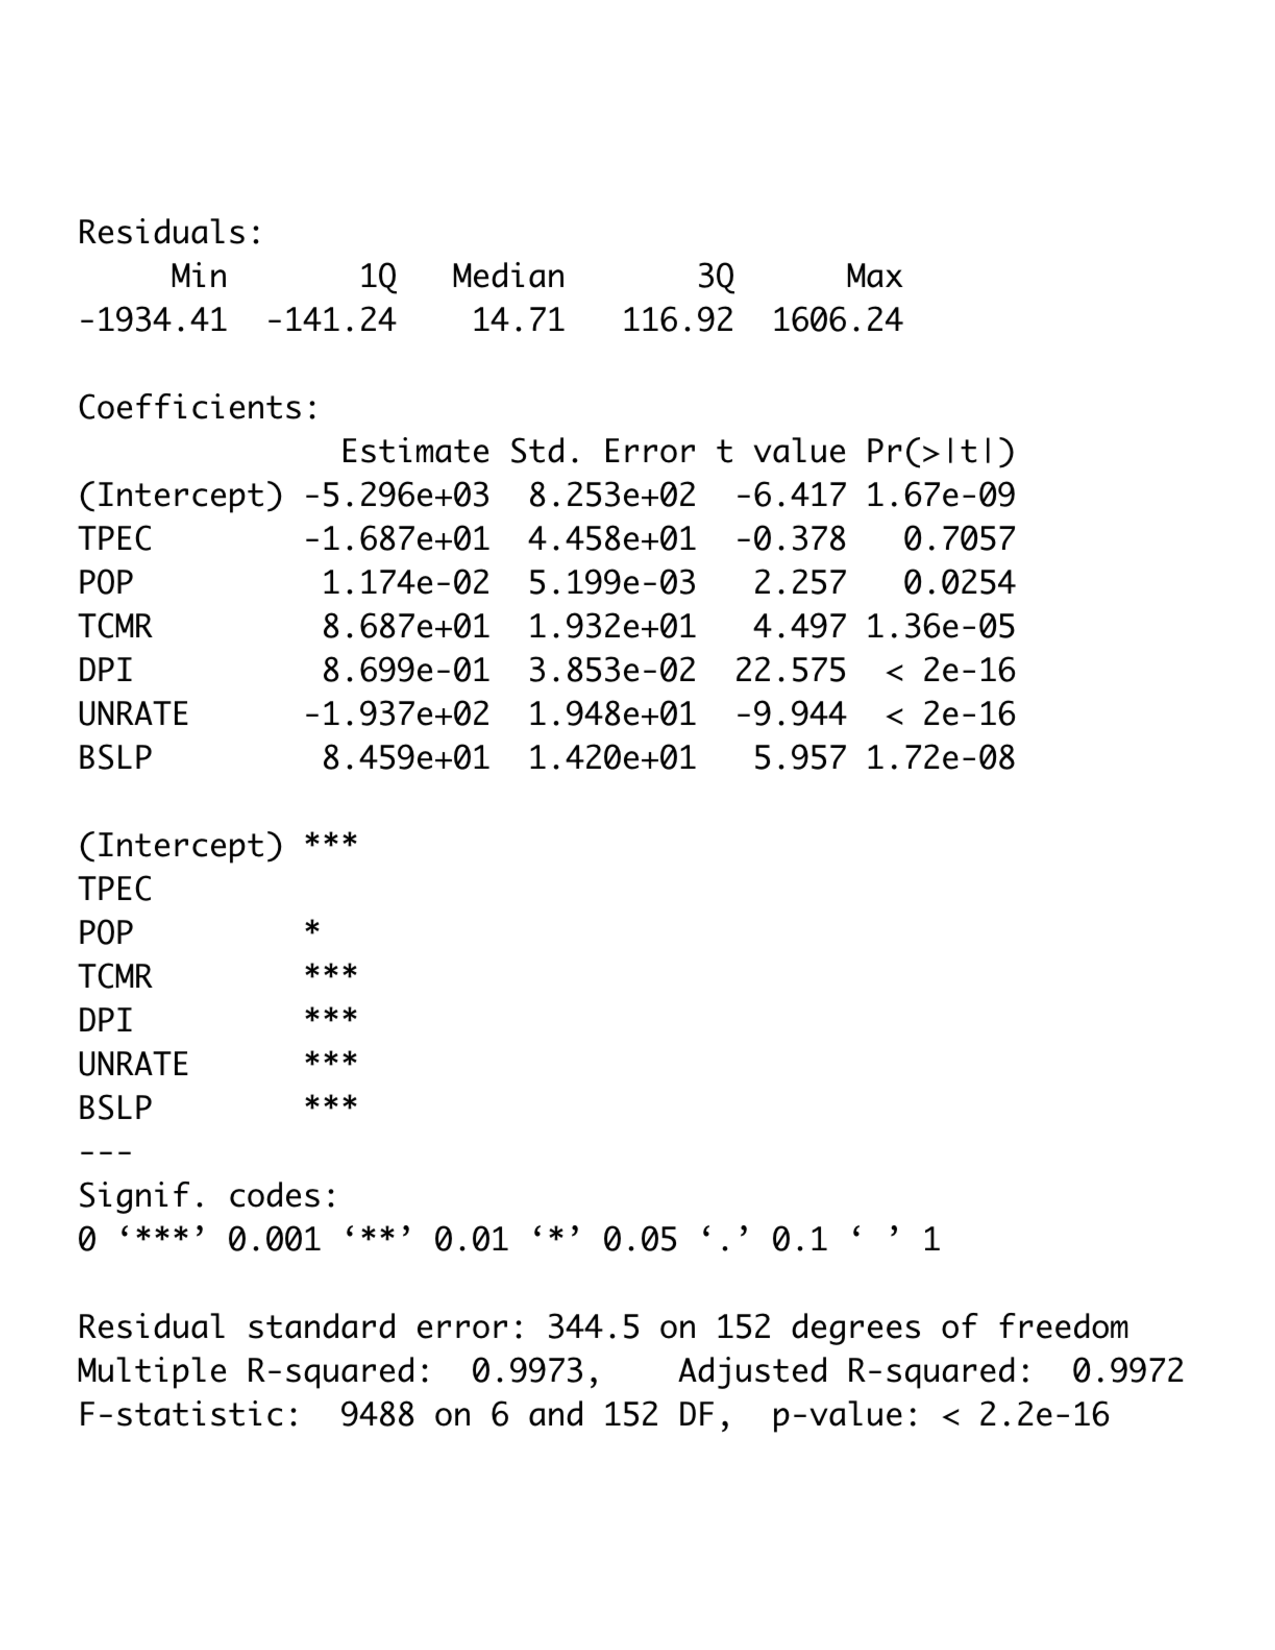
\includegraphics[scale = .35]{mod1output}
  \caption{This figure shows the output from R for the summary statistics for Model 1}
\end{figure}
From the output of Model 1, it concludes that the model is useful.
This is because the P-Value of the F-Test is less than $2.2 * 10^{-16}$.
The variables TCMR, DPI, UNRATE and BSLP are significant in this model, whereas the variables TPEC and POP are not significantly differnt from zero at the 5\% level of significance.  
The Multiple R-Squared value indicates that this model is a good fit since 99.73\% of the variablity in the data is explated by the model. 
Model 1 found significant relationships between the frequency of GDP and the variables TCMR, DPI, UNRATE and BSLP. 
This is due to P-Value associated with these variables is less than .001. 
Specifically it found a 86.87\% increase in the frequency of GDP for every 1\% increase in TCMR, a 86.99\% increase in the frequency of GDP for every 1\% increase in DPI, a -19.37\% decrease in the frequency of GDP for every 1\% increase in UNRATE, and a 84.59\% increase in the frequency of GDP for every 1\% increase in BSLP.
The Added Variable Plots for the model are as follows:
\begin{figure}[H]
  \centering
  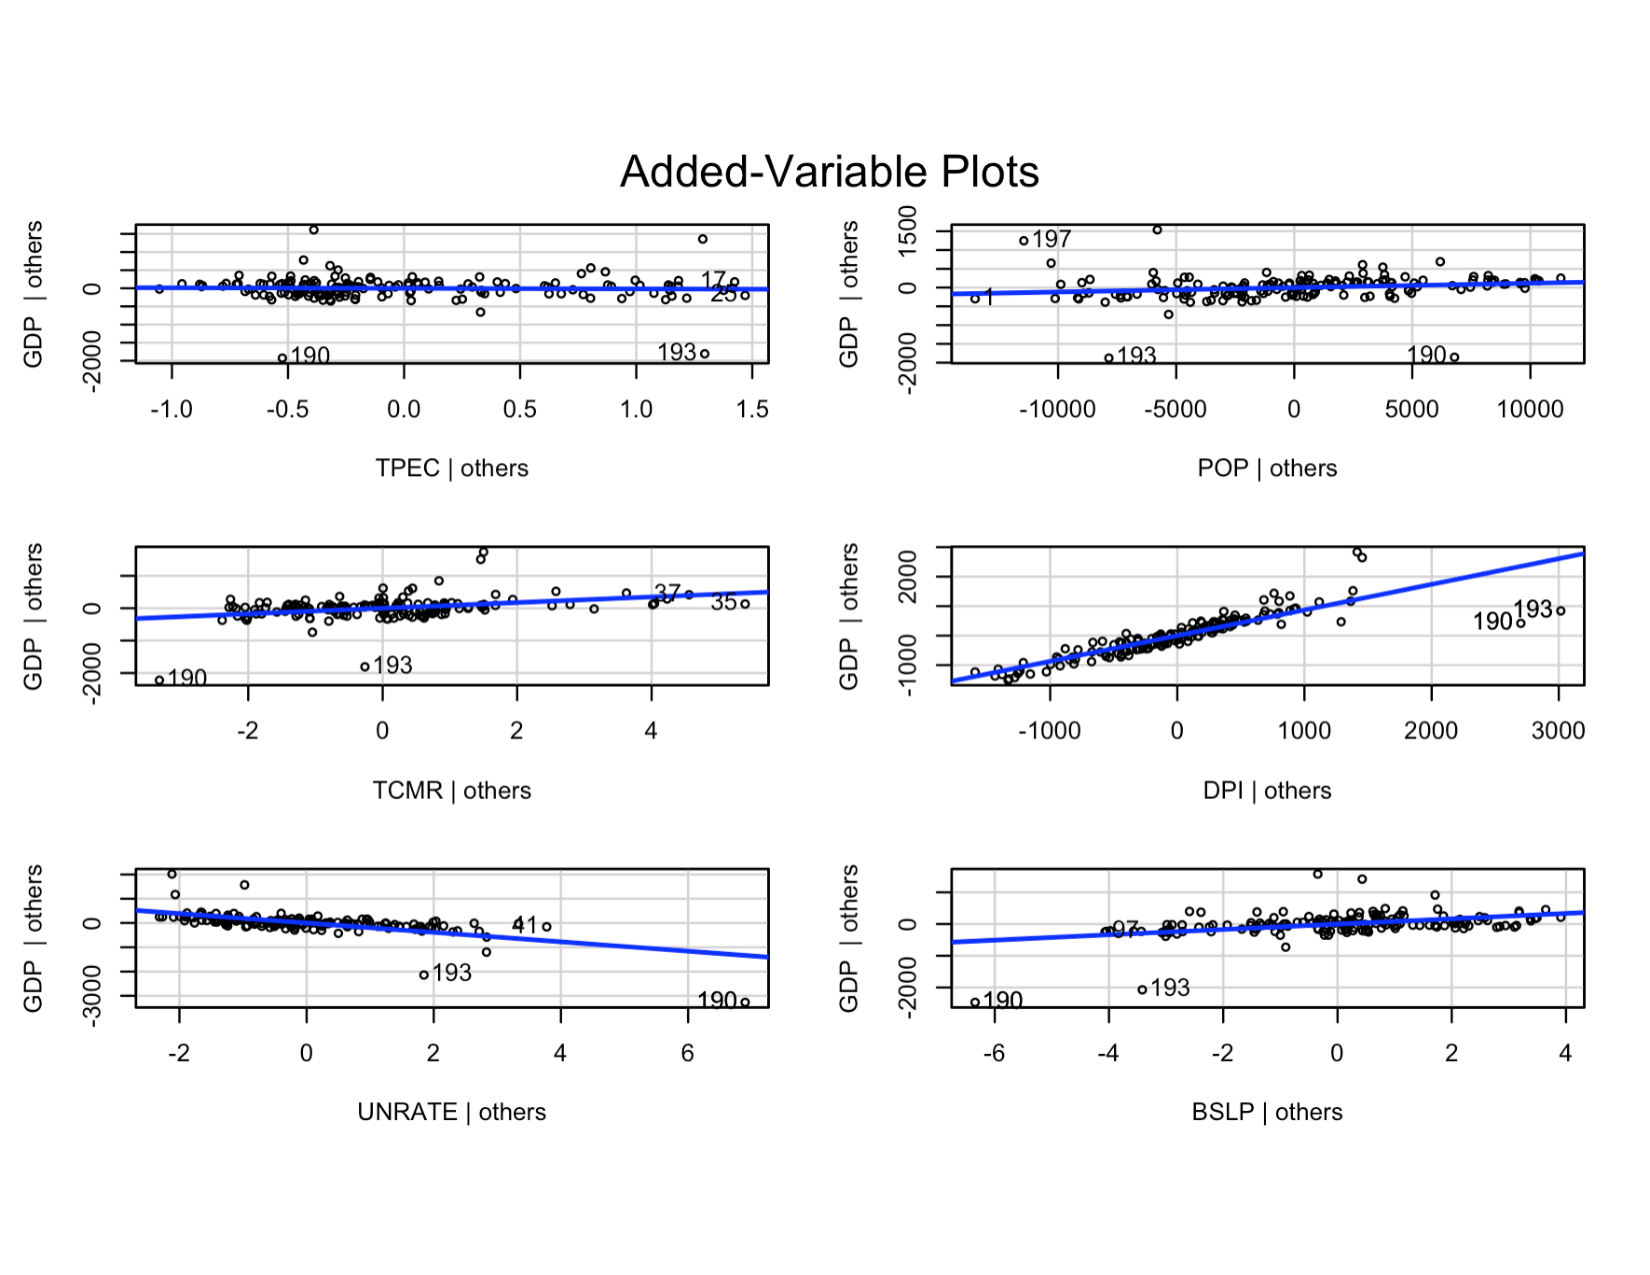
\includegraphics[scale = .35]{AVP1}
  \caption{This figure shows the AV Plots for the variables included in Model 1}
\end{figure}
From the output above, it can be concluded that there is a strong linear relationship between the variables TCMR, DPI, UNRATE and BSLP with GDP.
A weak linear relationship is show fromthe varibles TPEC and POP with GDP. 
This output confirms that the relationship between TPEC and POP with GDP are not significant in this model. 
To check the assumptions of homoscedacity a residuals vs. fitted plot is shown.
\begin{figure}[H]
  \centering
  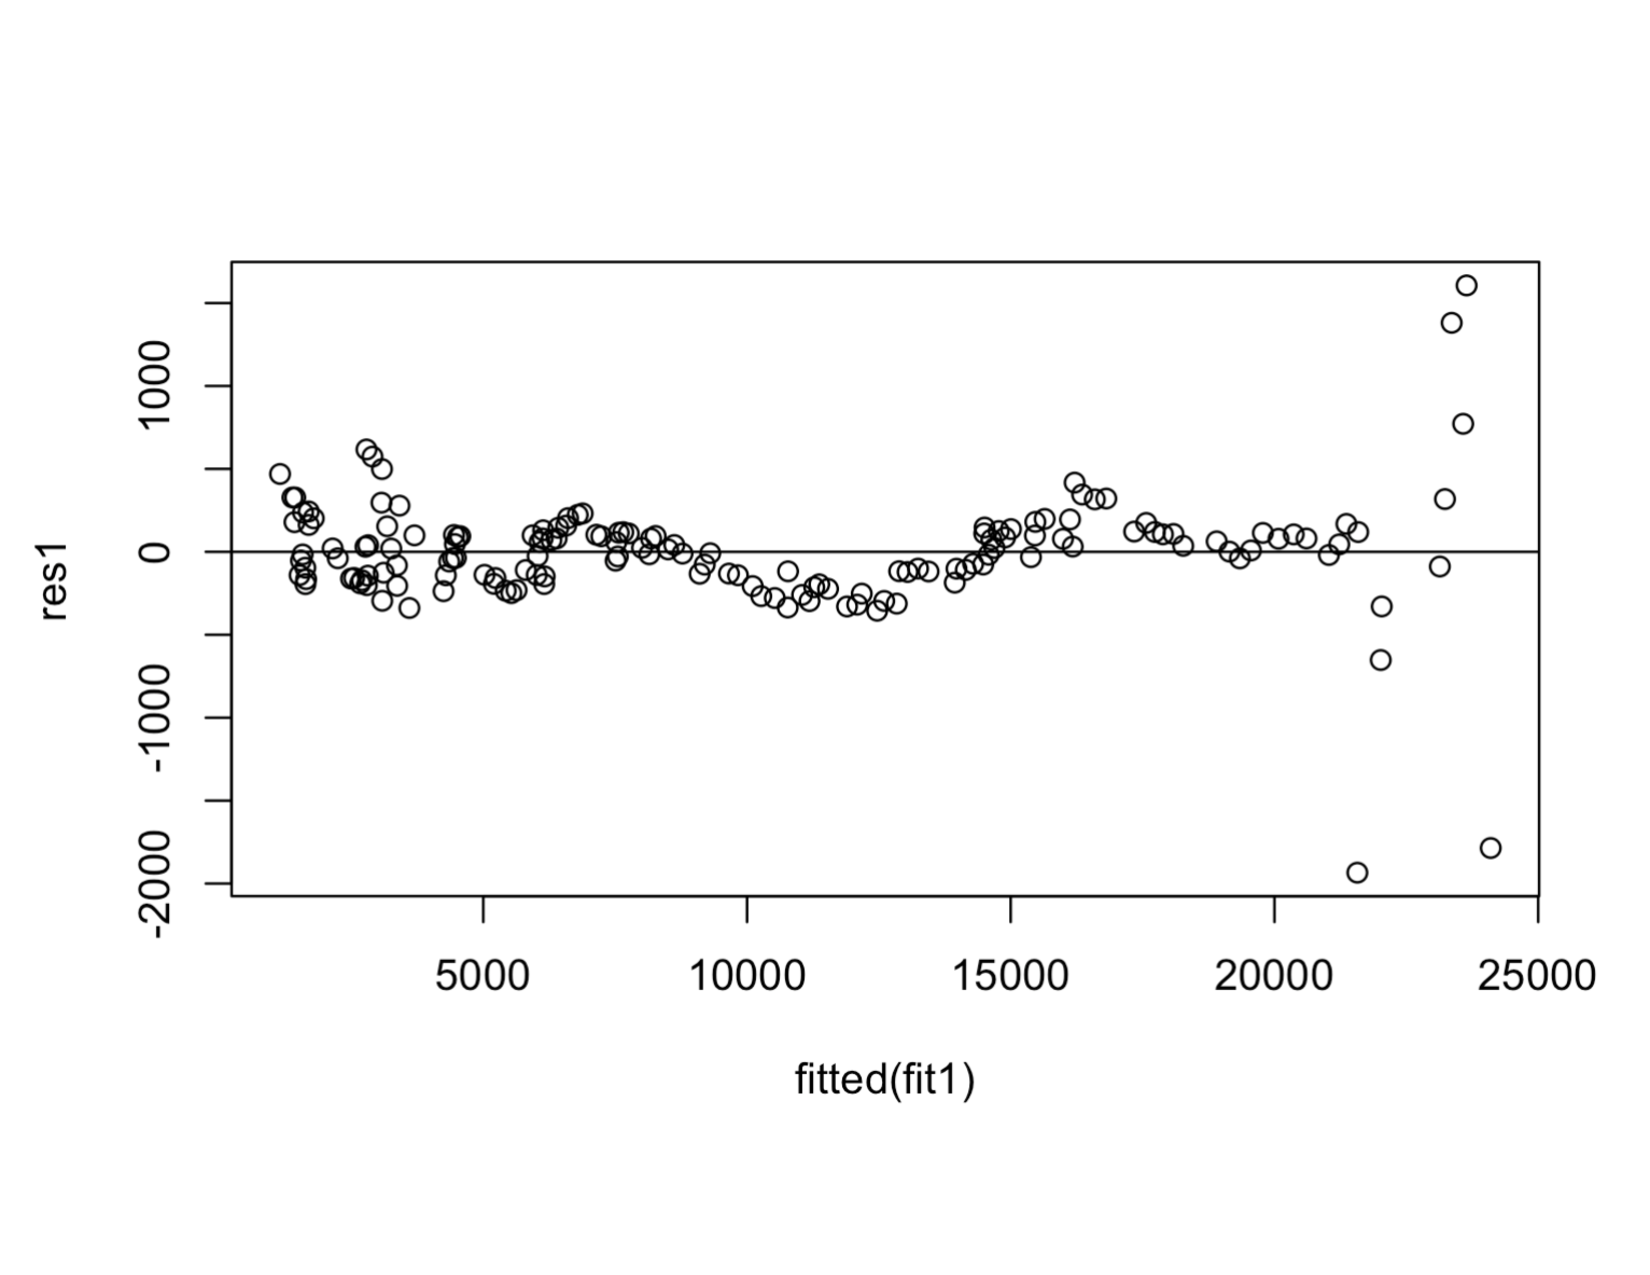
\includegraphics[scale = .35]{res1}
  \caption{This figure shows the Residuals vs. Fitted plot for Model 1}
\end{figure}
From this plot, the assumption of homoscedacity is questionable. 
The residuals do not appear to be randomly scattered throughout the entire plot, and there could be a noticle pattern. 
This warrents further invesigation. Next, the assumption of normality will be checked using a Q-Q Plot. 
\begin{figure}[H]
  \centering
  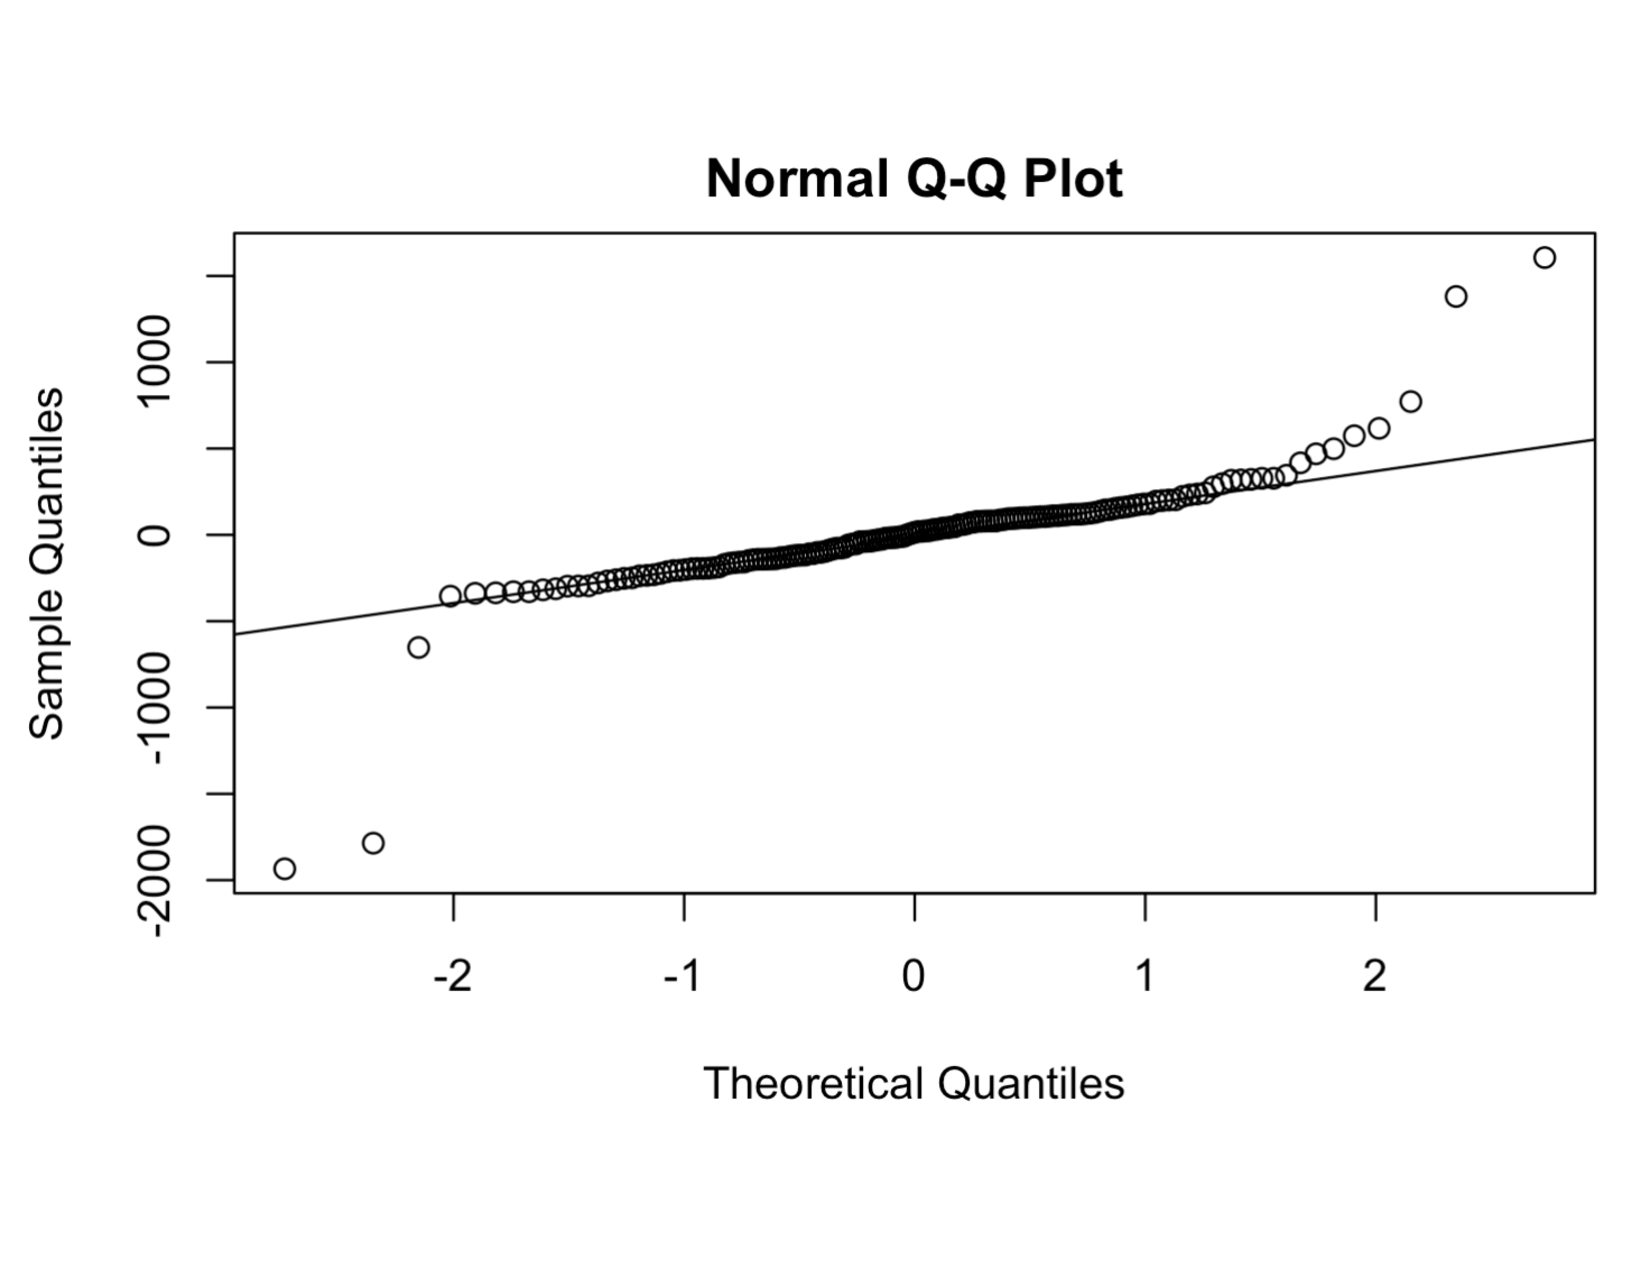
\includegraphics[scale = .35]{norm1}
  \caption{This figure shows the Q-Q Plot for Model 1}
\end{figure}
From this plot, the assumption of normality is met. 
The points fall along the line at a rough 45 degree angle. 
There is a few stray points, but not enough concern that warrents futer invesigation.
Therefore, the normality assumption is met. 

For the second model, the non significant variables from Model 1 are removed. 
Model 1 was built using the independent variables TCMR, DPI, UNRATE and BSLP from the training dataset. 
The equation used for Model 2 is as follows:
\begin{equation}
  GDP = \beta_0 + \beta_1TCMR+ \beta_2 DPI + \beta_3 UNRATE + \beta_4 BSPL
\end{equation}
Summary statistics for Model 2 are as follows:
\begin{figure}[H]
  \centering
  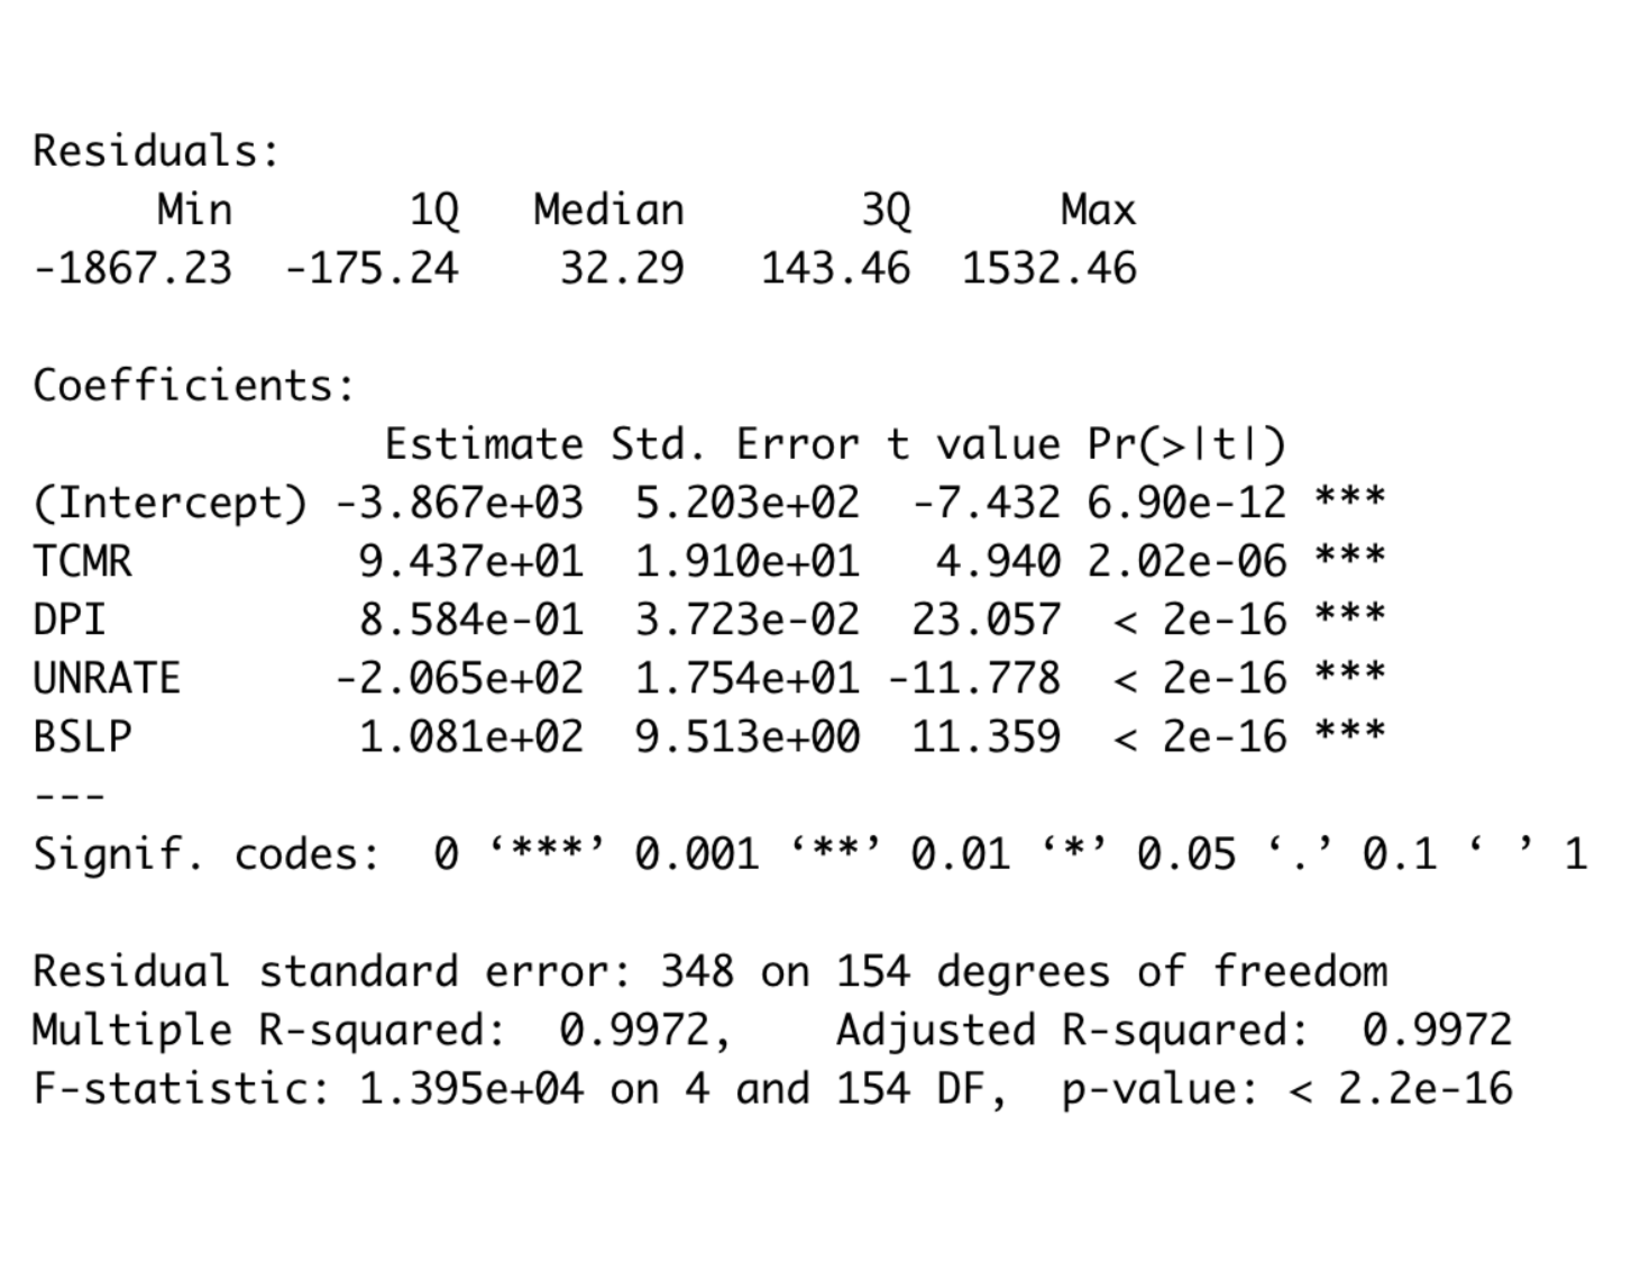
\includegraphics[scale = .35]{mod2output}
  \caption{This figure shows the output from R for the summary statistics for Model 2}
\end{figure}
From the output above of Model 2, it concludes that the model is useful.
This is because the P-Value of the F-Test is less than $2.2 * 10^{-16}$.
All of the variables in this model (TCMR, DPI, UNRATE and BSLP) are significant at the 5\% level of significance.
The R-Squared value indicates that this model is a good fit since 99.72\% of the variablity in the data is explated by the model. 
Model 2 found significant relationships between the frequency of GDP and the variables TCMR, DPI, UNRATE and BSLP. 
This is due to P-Value associated with these variables is less than .001. 
Specifically it found a 94.37\% increase in the frequency of GDP for every 1\% increase in TCMR, a 85.84\% increase in the frequency of GDP for every 1\% increase in DPI, a -20.65\% decrease in the frequency of GDP for every 1\% increase in UNRATE, and a 10.81\% increase in the frequency of GDP for every 1\% increase in BSLP.
The Added-Variable Plots for variables included in Model 2 are as follows: 
\begin{figure}[H]
  \centering
  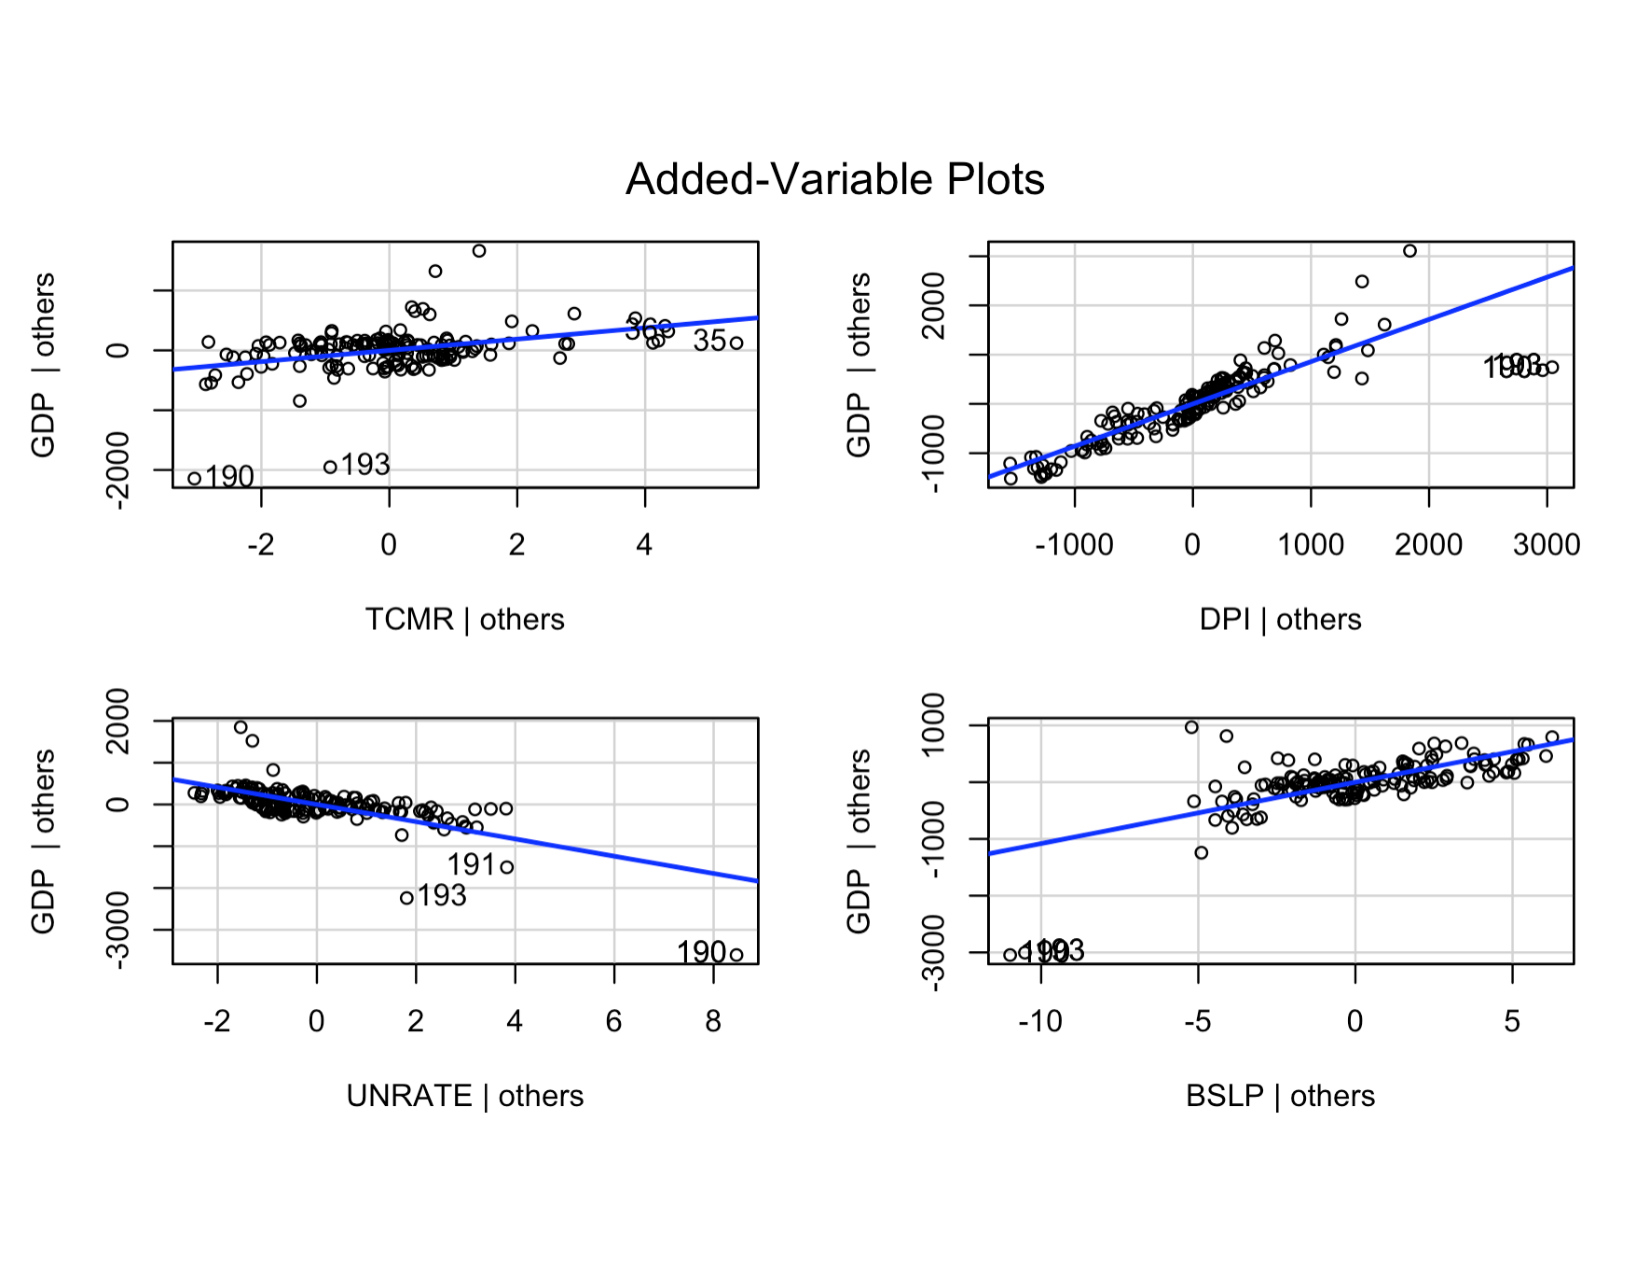
\includegraphics[scale = .35]{AVP2}
  \caption{This figure shows the AV Plots for the variables included in Model 2}
\end{figure}
From the output produced in the Added-Variable Plots from Model 2, it confirms there is a strong linear relationship between the variables TCMR, DPI, UNRATE and BSLP with GDP. 
To check the assumptions of homoscedacity a residuals vs. fitted plot is shown.
\begin{figure}[H]
  \centering
  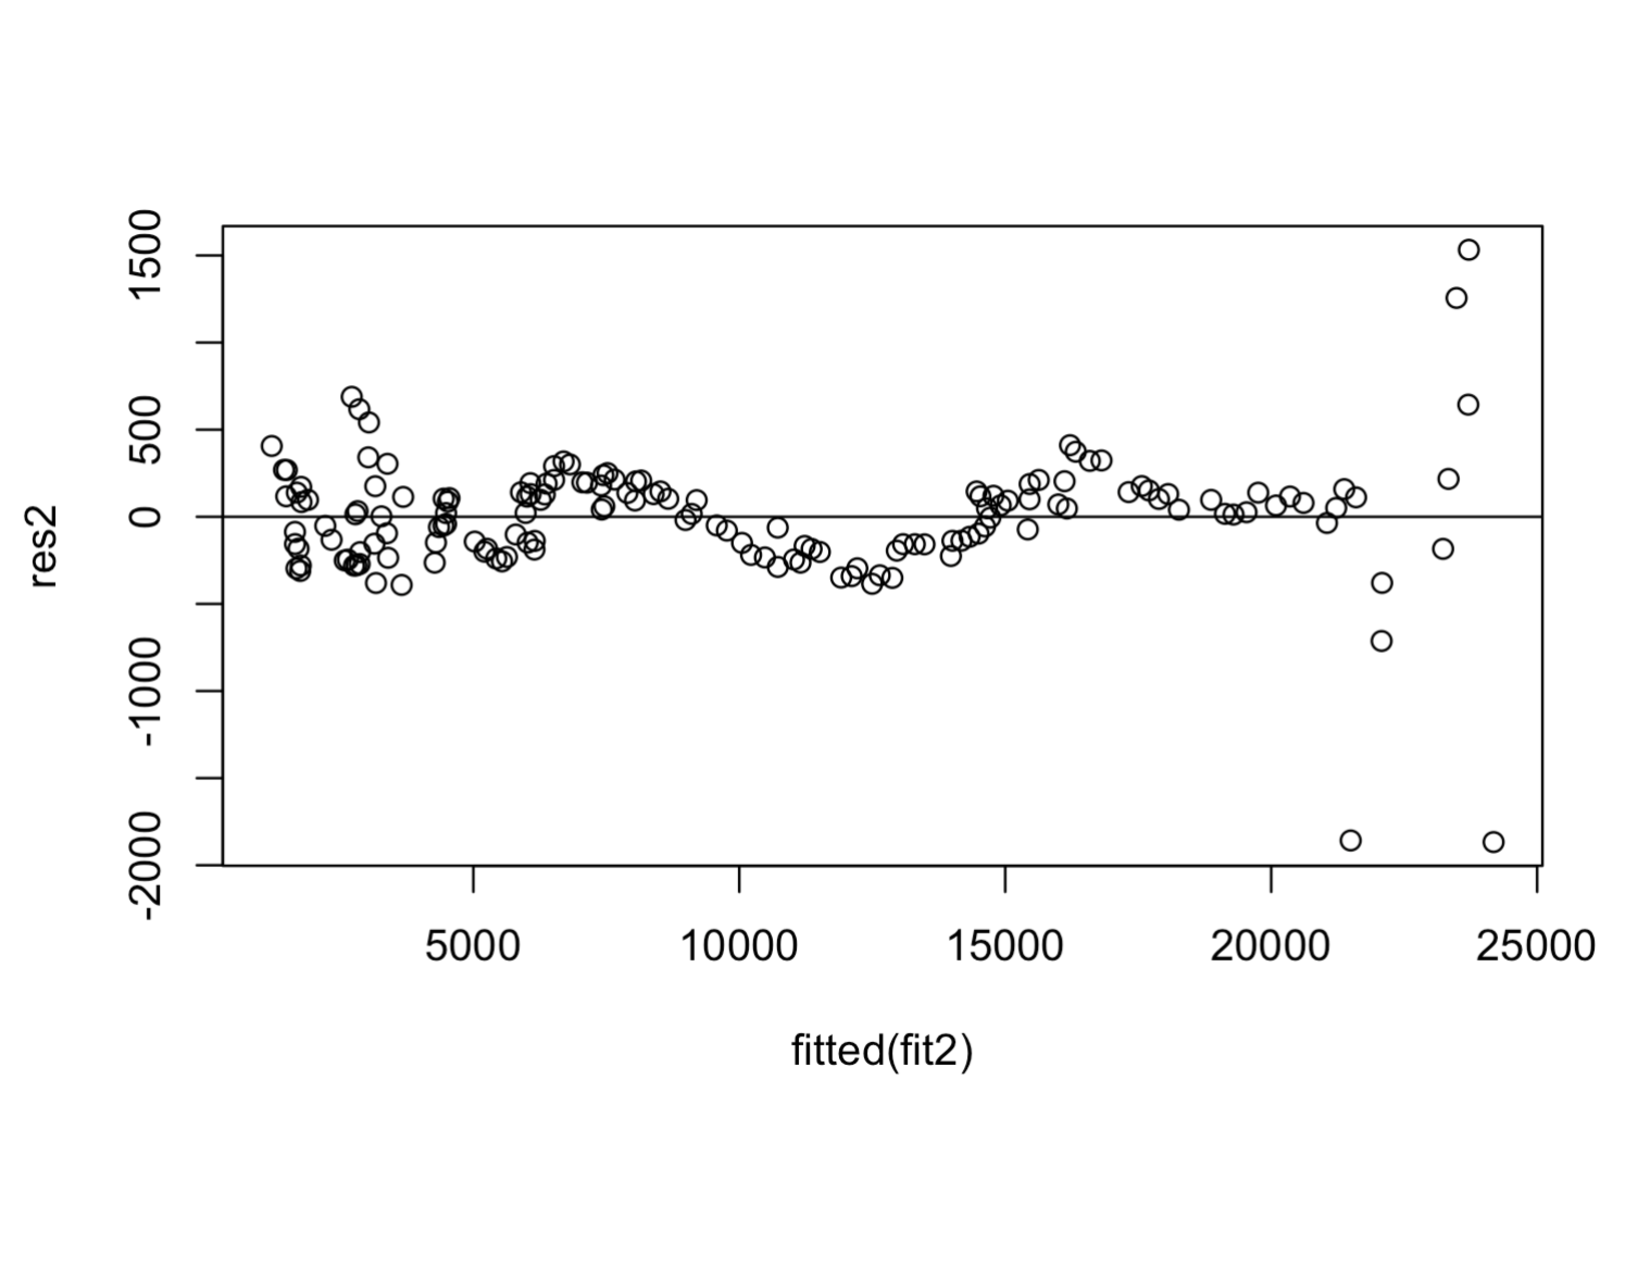
\includegraphics[scale = .35]{res2}
  \caption{This figure shows the Residuals vs. Fitted plot for Model 2}
\end{figure}
From this plot, the assumption of homoscedacity is questionable
The residuals do not appear to be randomly scattered throughout the entire plot, and there could be a noticle pattern in some parts of the plot. 
This warrents further invesigation. 
Next, the assumption of normality will be checked using a Q-Q Plot. 
\begin{figure}[H]
  \centering
  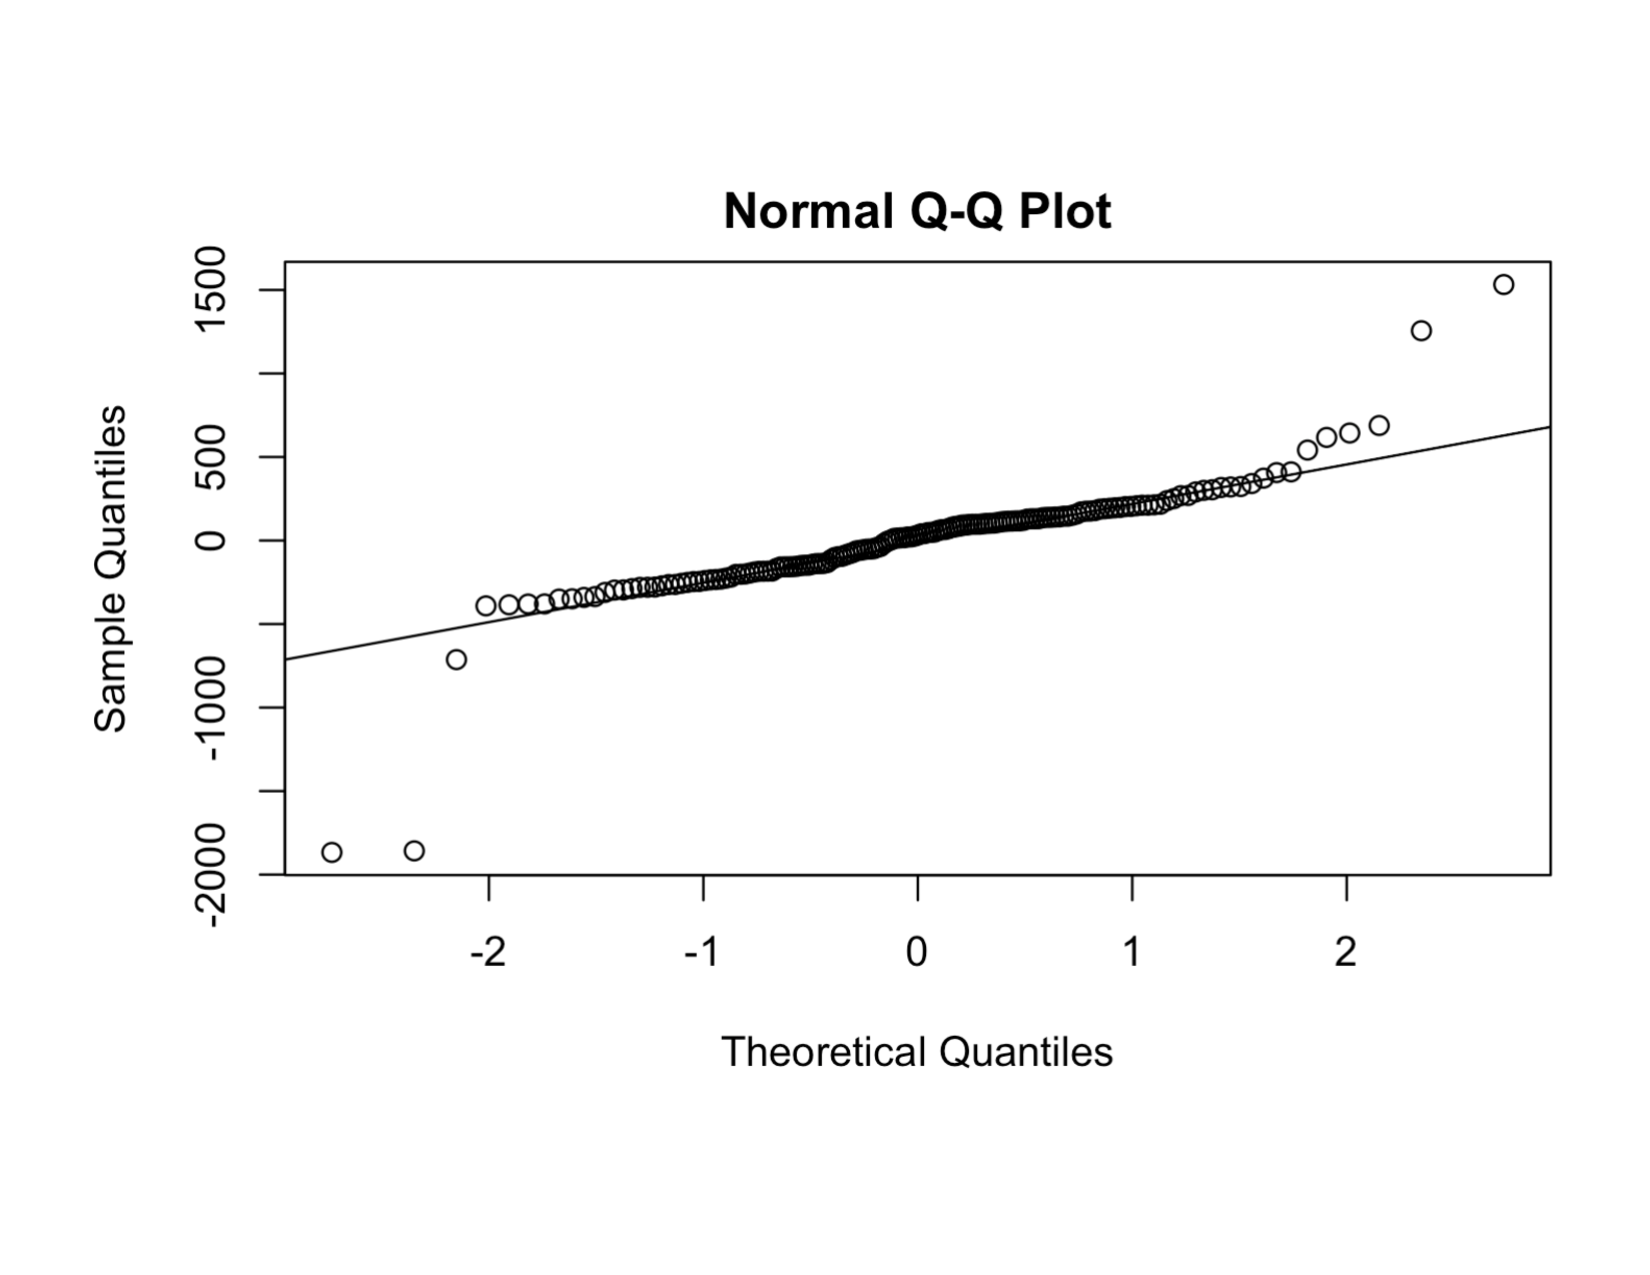
\includegraphics[scale = .35]{norm2}
  \caption{This figure shows the Q-Q Plot for Model 2}
\end{figure}
From this plot, the assumption of normality is met. 
The points fall along the line at a rough 45 degree angle. 
There is a few stray points, but not enough concern that warrents futer invesigation.
Therefore, the normality assumption is met. 

Next, the validation data will be applied to Model 1 and Model 2. 
The summary statistics for Model 1 application with Validation data are as follows: 
\begin{figure}[H]
  \centering
  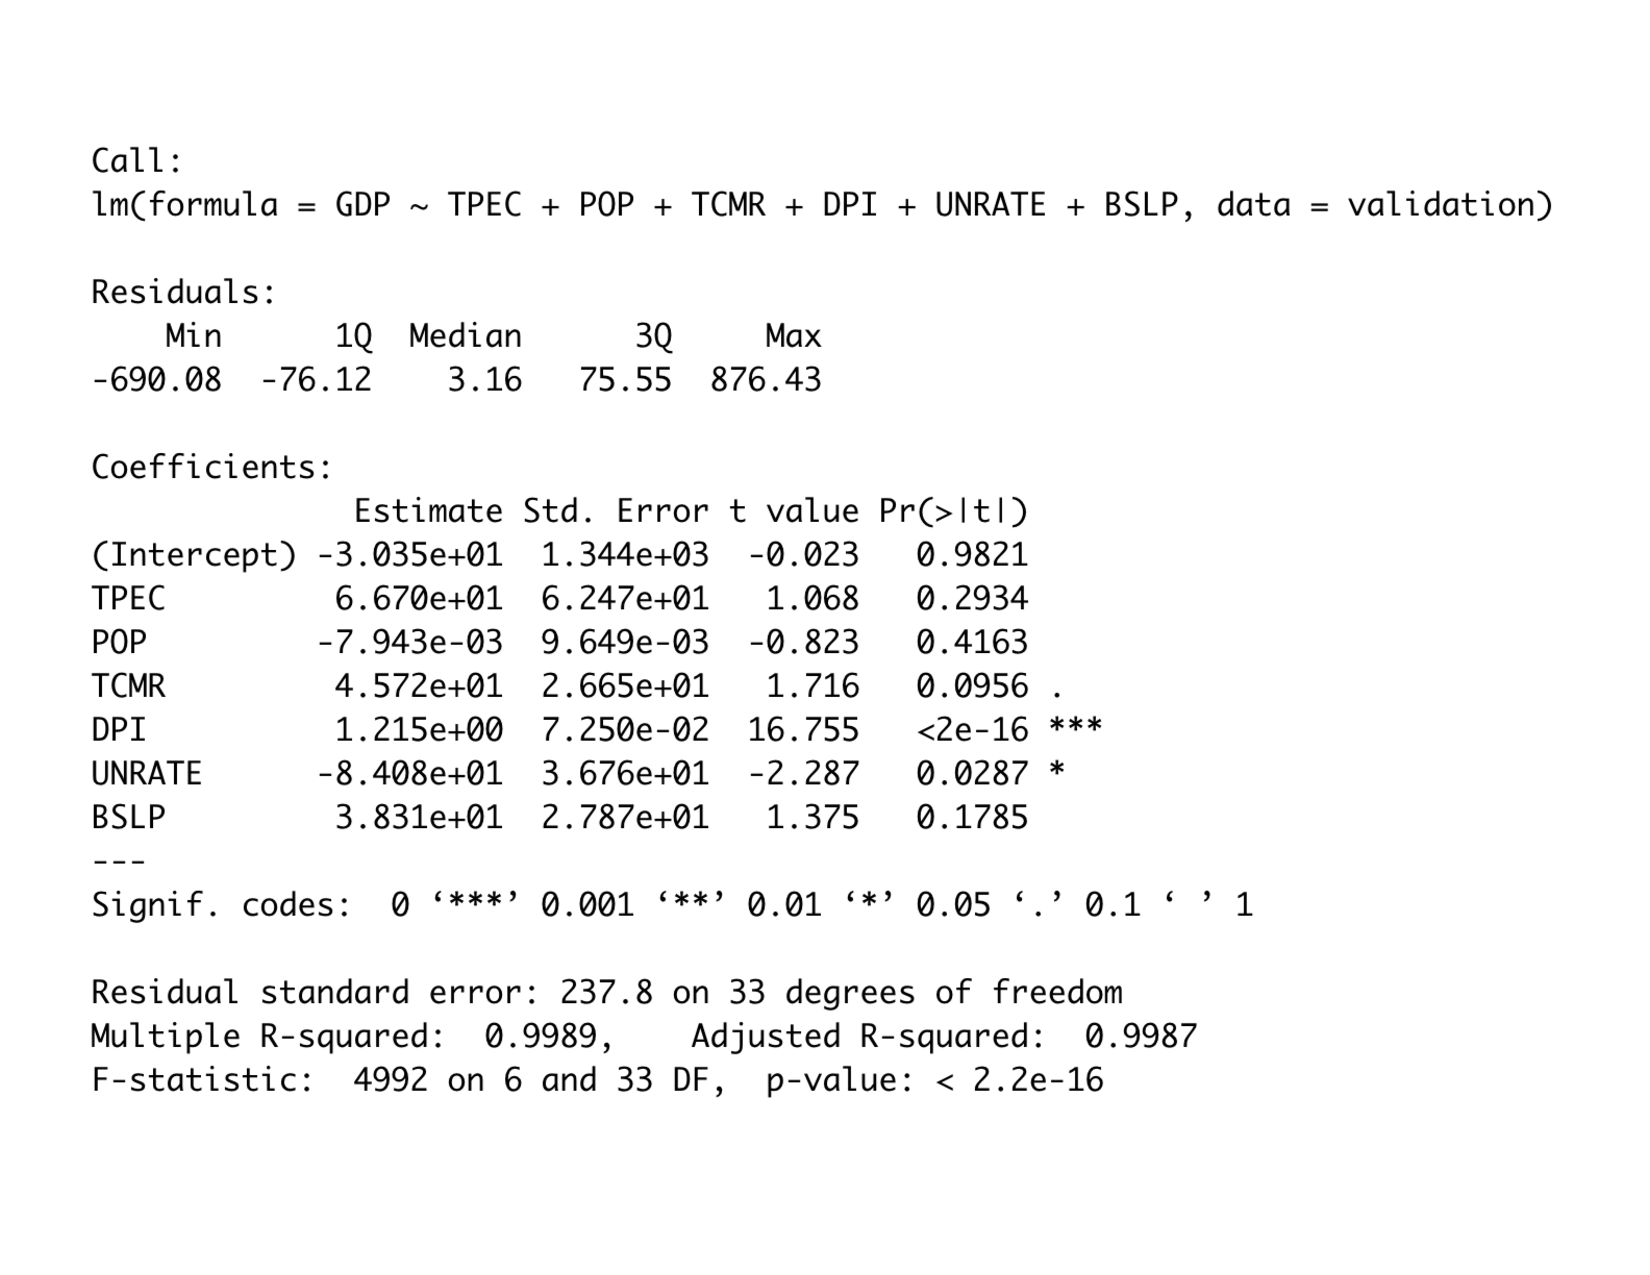
\includegraphics[scale = .35]{mod1v}
  \caption{This figure shows the summary statistics for Model 1 application to the validation dataset.}
\end{figure}
The summary statistics for Model 2 application with Validation data are as follows: 
\begin{figure}[H]
  \centering
  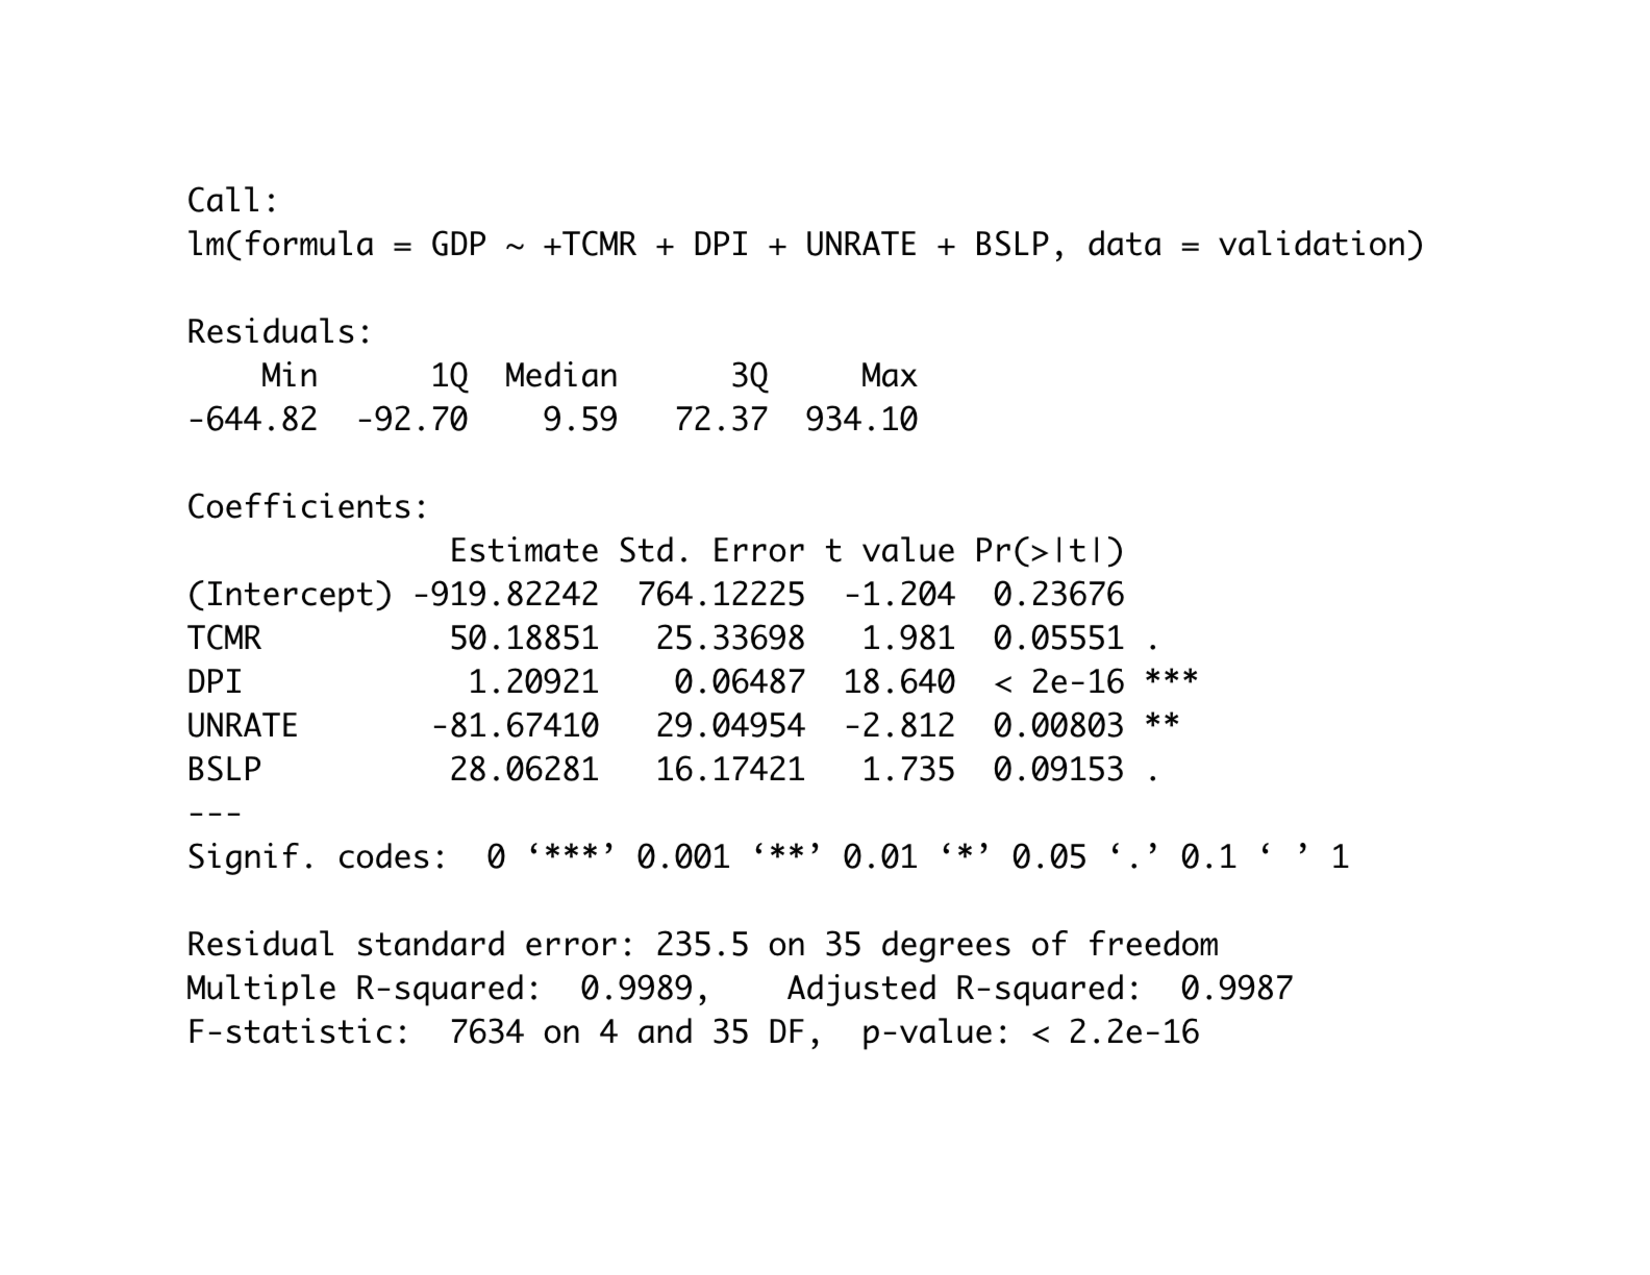
\includegraphics[scale = .35]{mod2v}
  \caption{This figure shows the summary statistics for Model 2 application to the validation dataset.}
\end{figure}

Next, and AIC test will be applied to Model 1 and Model 2 application to validation data. 
This tested resulted in Model 1 reciving and AIC of 559.5405, and Model 2 557.1234. 
Since Model 2 recived a lower AIC. 



\section*{Discussion}


- violate homoscedacty assumption

\bibliography{refrences}
\bibliographystyle{chicago}

\end{document}